\documentclass[technical_document.tex]{subfiles}
\begin{document}

Eva\textquotesingle{}s arm was designed with a focus on minimizing production time\footnote{Just one month was planned as production time, to leave some time for testing}. %TODO reference design constrains from the paper?
Two independent 3D drawings were made using CAD software\footnote{Solidworks was used as the main CAD program for all mechanical parts}. These designs gave a good overview of the required parts and were helpful in estimating the production time. The idea was to divide the arm into small parts thata re easy to manufacture. This wa even during a relatively short time (for example, if the workshop was only available for a few hours), at least one part could be made. Parts with wrong dimensions or other manufacturing errors could be replaced fairly quickly, as the production time per part is very low. 
These parts were created with more and more detail, in an iterative process. Parts that would be too complex were divided into smaller and simpler parts. In the CAD software these parts were connected to form the arm, including all necessary bolts and nuts. When all parts were finished, this main assembly was tested for interfering parts and possibility of assembling. Most parts are made from aluminium, since it is a lightweight and easily available material. Small shafts or connectors were mostly created from steel, since they generally have high stress concentrations on them. Furthermore, due to their small dimensions the extra weight is minimal. The assumptions about material choice have been validated using numerous calculations, as will be discussed later.

\section{Design of the arm}

Most important part of the robotic arm is the shoulder. It has to support the weight of the whole arm including the object in the gripper and should be strong and stiff enough for the gripper to be placed accurately, even when accelerating.

\begin{figure}[ht!]
	\centering
	\mbox{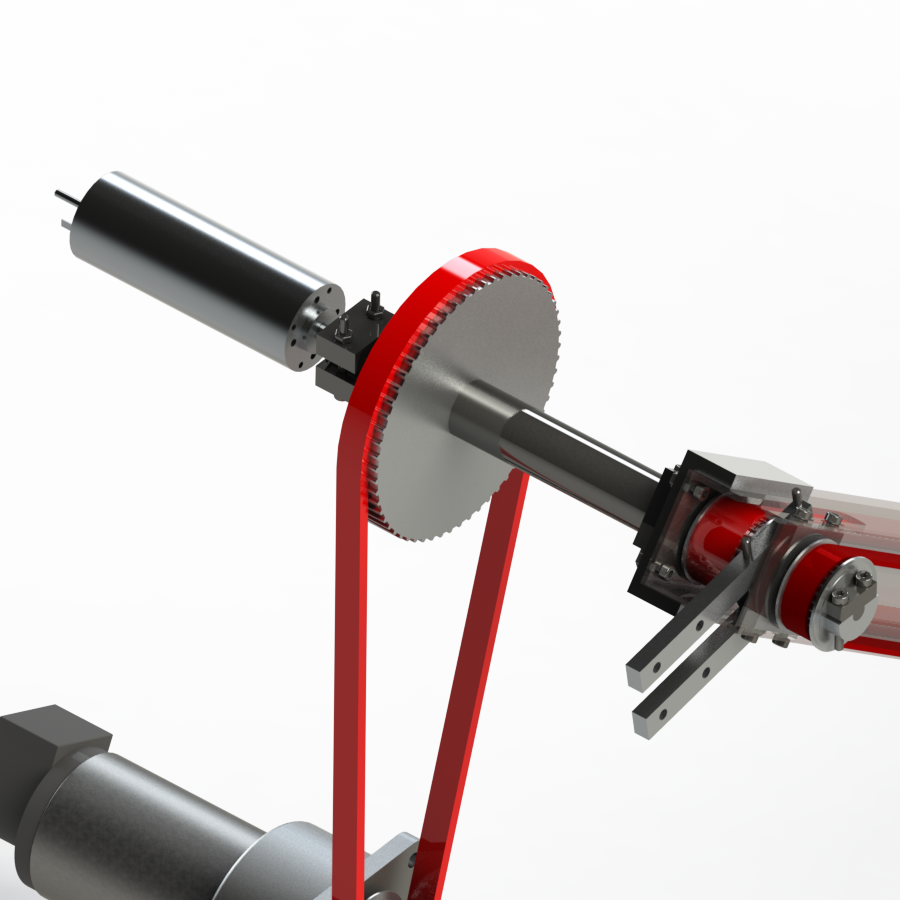
\includegraphics[scale=1.0]{Images/arm_shoulder.png}}
	\caption{Shoulder joint of Eva\textquotesingle{}s arm}
	\label{fig:arm_shoulder}
\end{figure}

The main idea is very simple. The upper arm can move up and down, like a simplified shoulder. Further down the arm is the elbow, whick makes sure the lower arm is always horizontal. The last part of the arm can move sideways. An overview of Eva\textquotesingle{}s arm is shown in fig. \ref{fig:overview}.

The upper arm is a standard square tube, connected to a hollow shaft. The shaft is supported by a set of bearings, resulting in an upper arm that can move freely in just one direction. The arm is moved by driving the shaft via a timing belt. There is a second motor located close to the shoulder, which drives the sideways motion of the arm. This is done via a small axis located within the main shoulder shaft, driving the lower arm via a set of timing belts. This second motor and especially its shaft running through the shoulder make this joint the most complex one. Another important thing to notice is the way the bearing mounts are connected to the upper arm. They are designed in such a way that just by re-tightening a few bolts, the tension on the belts can be adjusted.

From the shoulder to the elbow joint, the arm basically consists of a standard 40x40x2mm beam. The interesting part is how it links the elbow joint to the body. Inside the upper arm is another timing belt, connecting the elbow to a solid part of the shoulder. This ensures the lower arm is always in the same direction relative to the body. In this case the lower arm is always horizontal, as this is the most practical configuration for grasping objects from a table. Driving the inner timing belt with a motor instead of keeping it fixed to the body would make the lower arm capable of turning independently, adding another degree of freedom. This would be a relatively easy modification, as only a few changes are required in the shoulder. It would, however, make the arm slightly more difficult to control.

\begin{figure}[ht!]
	\centering
	\mbox{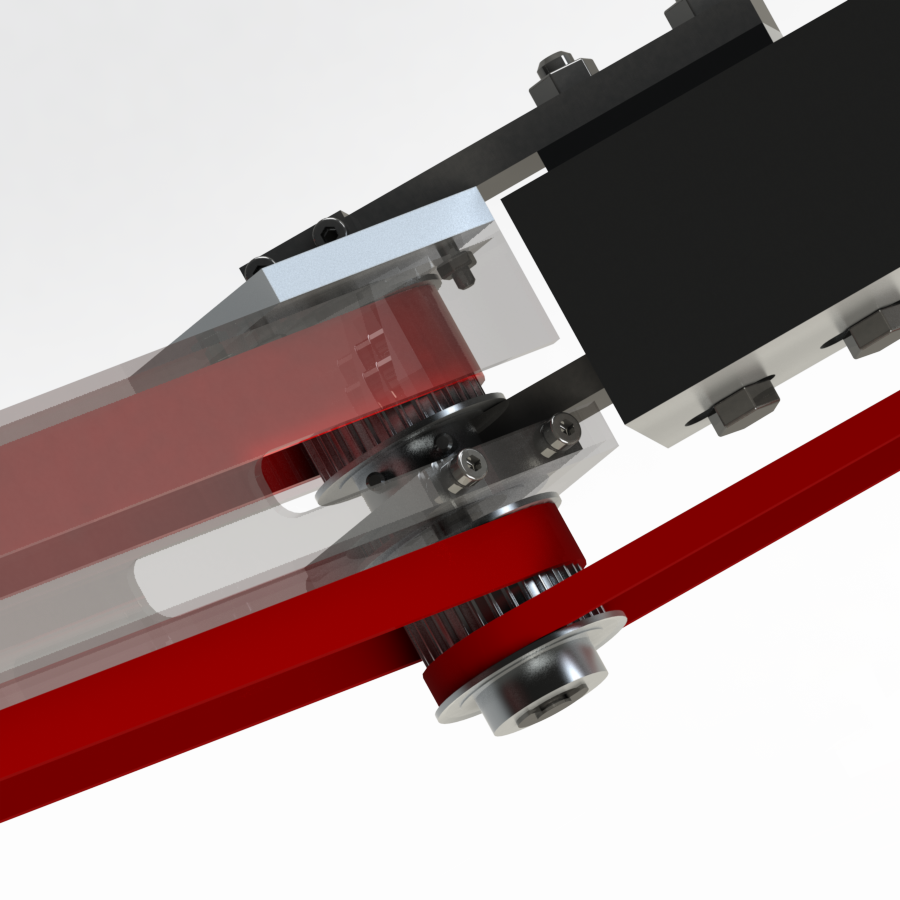
\includegraphics[scale=1.0]{Images/arm_elbow.png}}
	\caption{Elbow joint of Eva\textquotesingle{}s arm}
	\label{fig:arm_elbow}
\end{figure}

The elbow joint itself is fairly simple. The inner timing belt connects to a pulley, which is directly screwed onto the lower arm. This ensures the lower arm follows the reference angle given by the shoulder, as described earlier. The pulley is suspended by two bearings, connected to the upper arm via bearing mounts. Note these mounts are fixed in place, since the belt tension can be adjusted on the other end. The extra pulley on the outside of the joint is on the same shaft as the other pulley, but this one is free to turn independently of the shaft. The only purpose of this pulley is passing the rotation from the upper belt to the lower belt. This belt will eventually drive the sideways motion, as will be discussed in the next paragraph. The lower arm consists of the parts connected to the pulley and the beam itself. These are connected to each other in a way that allows adjusting the tension on the lower belt.

\begin{figure}[ht!]
	\centering
	\mbox{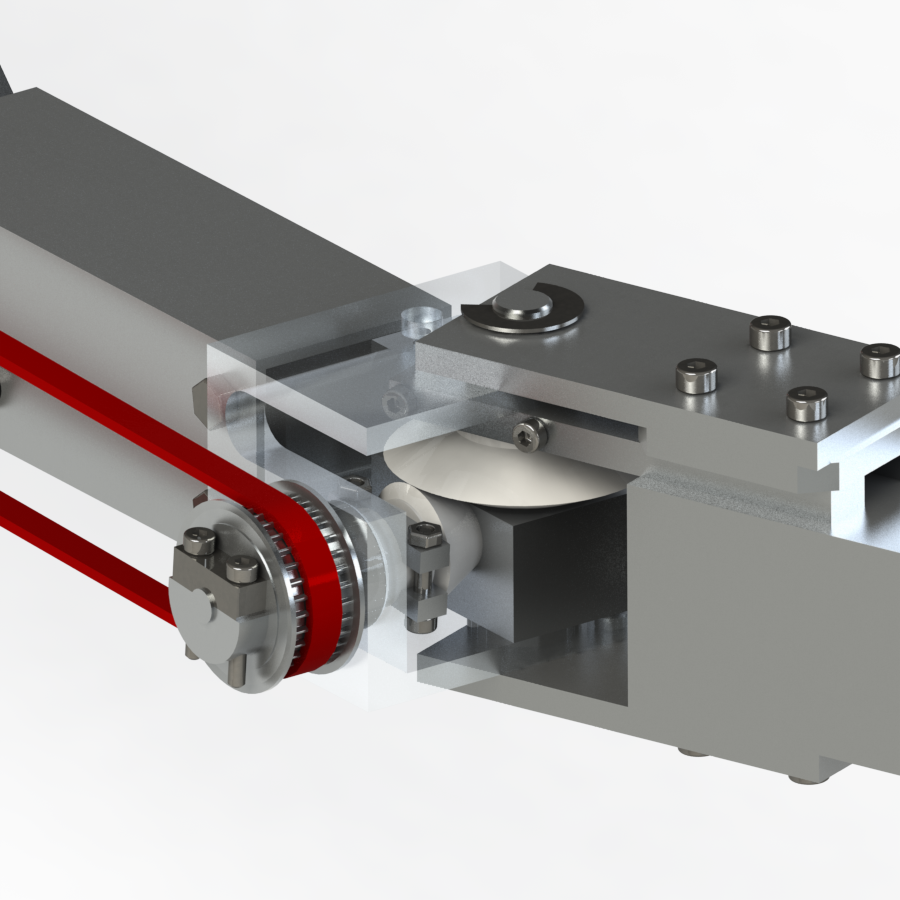
\includegraphics[scale=1.0]{Images/arm_sideJoint.png}}
	\caption{Sideways joint of Eva\textquotesingle{}s arm}
	\label{fig:arm_sideJoint}
\end{figure}

The last moving joint in the arm is the ‘sideJoint’: it allows Eva to move her arm a bit sideways. In a human arm, this direction of movement is integrated in the elbow, but Eva has a separate joint for this. The length of the link between those two joints is chosen based on the form of Eva\textquotesingle{}s body, so she can fold her arm in a compact way while driving or in standby mode. The motion is provided by the timing belt running on the outside of the arm. This belt drives a set of bevel gears to convert the rotation to the right direction. The bevel gears have a transmission ratio of 1:2, so the last link of the arm rotates with half the speed of the timing belt pulleys. This was done to makes the rotation less sensitive to play in the timing belts, lower the tension on the timing belts and simply because this set of gears is more compact than a comparable 1:1 set would be.

\begin{figure}[ht!]
	\centering
	\mbox{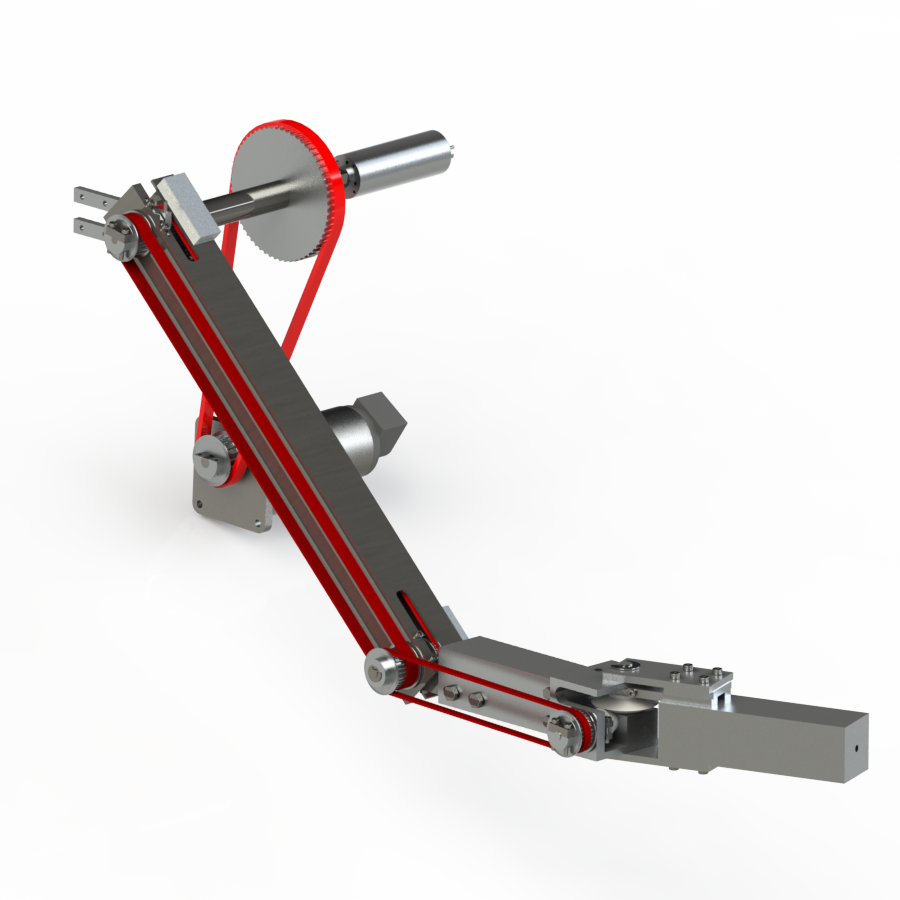
\includegraphics[scale=1.0]{Images/overview.png}}
	\caption{Overview of Eva\textquotesingle{}s arm}
	\label{fig:overview}
\end{figure}

The last part of the  arm is the gripper, connected to the ‘sideJoint’ via a standard beam. As the gripper design unfortunately is not open source, it was not possible to include it in the drawings. Linking all previously mentioned parts together, the total arm looks as in figure \ref{fig:overview}.


\section{Strength calculations}

Before production, Eva\textquotesingle{}s arm was subjected to a number of calculations to check its strength and stiffness. The most critical point turned out to be the shoulder, as this is a complex part where a lot of torque concentrates. Furthermore, the upper arm needs to resist twisting as the lower arm is capable of moving sideways, potentially producing a significant torque on the upper arm. After numerous calculations, by hand as well as assisted by our CAD program, the conclusion was that most parts were  strong enough for our needs, but some needed reinforcement. Especially the upper arm would be too weak if made from aluminium. This is the reason the upper arm is made out of steel. Steel is a lot heavier than aluminium, but as the mass centre of this part is pretty close to the shoulder, its impact on the inertia is limited.
Including calculations with their according free-body diagrams and Solidworks simulations would be very verbose, as over 25 different parts have been designed, some of which are used multiple times in different situations. Therefore, only the most critical (thus the most interesting) parts of Eva\textquotesingle{}s arm are being discussed in this section.

\begin{figure}[ht!]
	\centering
	\mbox{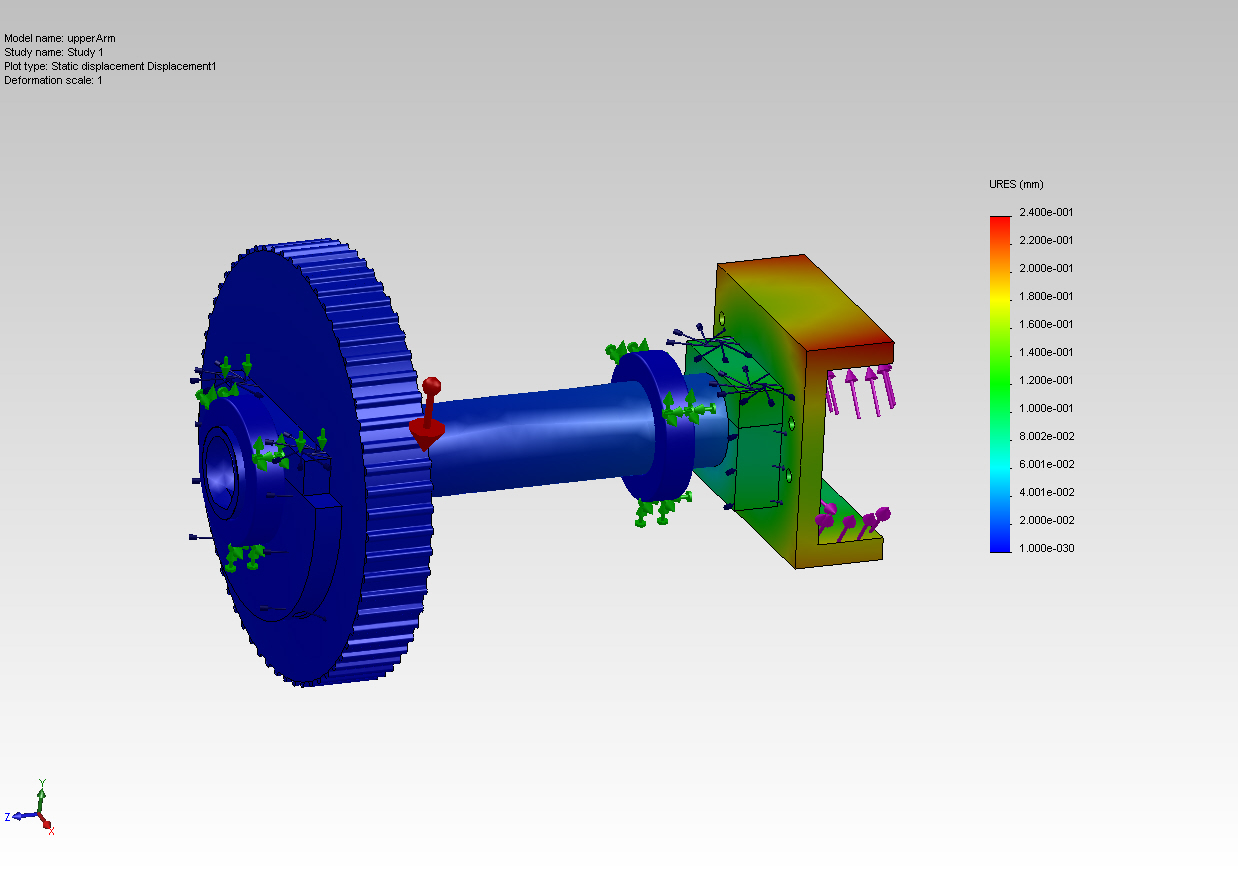
\includegraphics[scale=0.4]{Images/upperArm_displace.jpg}}
	\caption{Displacement plot of the shoulder}
	\label{fig:shoulder_displace}
\end{figure}

First point of interest was checking the shoulder mount. The weight of the arm and the object its grasps results in a torque around the shaft, as shown in \ref{fig:shoulder_displace} and fig.\ref{fig:shoulder_FOS}. The aluminium part connecting the arm with the shaft is the weakest point. Initially, this part was designed a bit too thin, resulting in large deformations and too much stress. Fig.\ref{fig:shoulder_displace} shows the deformation, where red is 0.2mm and blue is neutral. As expected, the corners displace the most from their original position, as a result of the torque. To see if the parts meet the strength requirements, a plot of the safety factor is shown in fig.\ref{fig:shoulder_FOS}

\begin{figure}[ht!]
	\centering
	\mbox{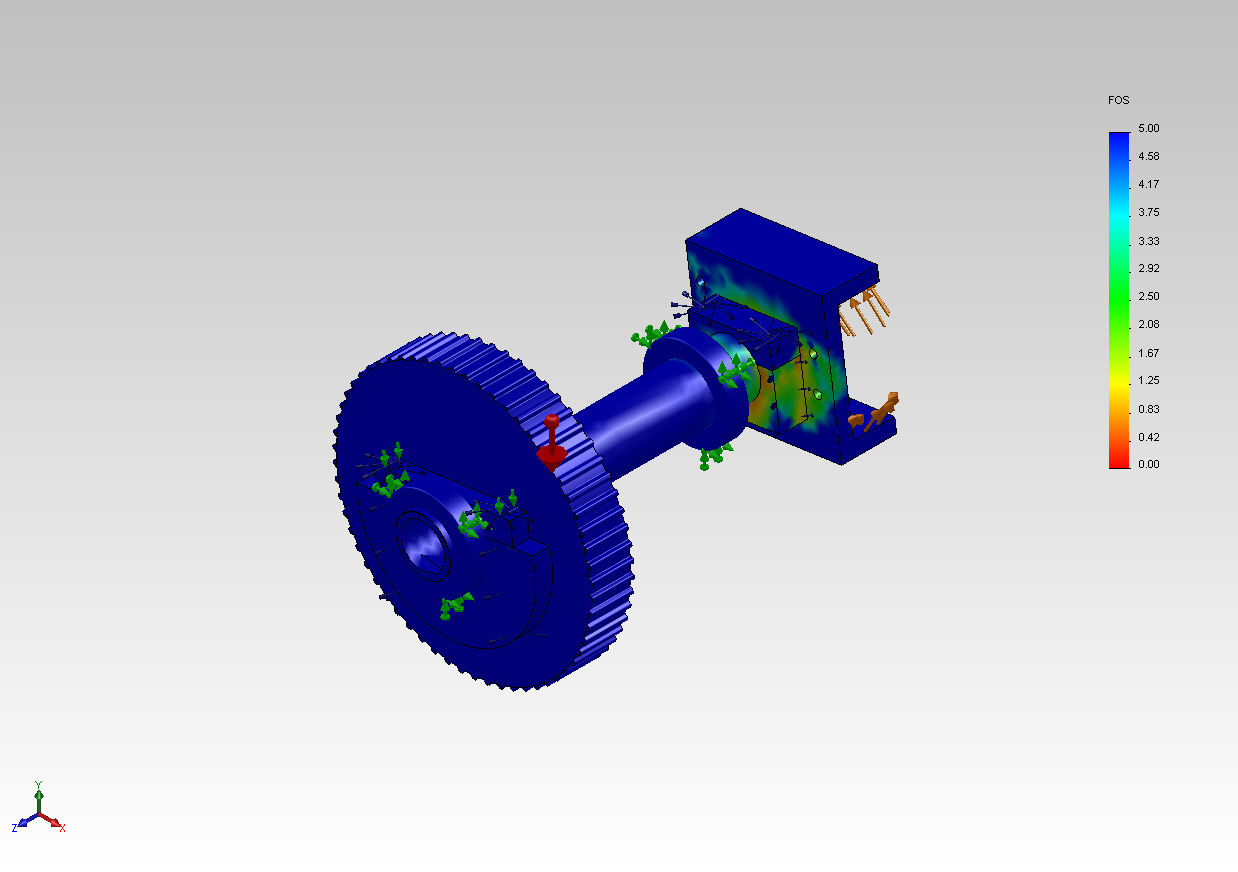
\includegraphics[scale=0.4]{Images/upperArm_FOS.jpg}}
	\caption{Factor of safety plot of the shoulder}
	\label{fig:shoulder_FOS}
\end{figure}

The factor of safety should be at least 1.0, as any value below indicates the part would probably break. The final design, as depicted in the figure, is strong enough. The factor of safety is generally above 5, but at some points it is around 1.0. These points are where all force concentrates on small areas or in close proximity of sharp corners.

Knowing the shoulder itself is strong enough, the upper arm is also of interest. Because of the large cuts in the arm, stress is expected to concentrate around its edges. The part was designed to be aluminium first, but the calculations showed it would be too weak. The beam in general is strong enough, but the edges of the cuts would certainly break. Its safety factor was below 0.5 and the stress was clearly higher than the aluminium would be able to take.Therefore steel was selected as material for the main beam of the upper arm. In fig.\ref{fig:upperArm_FOS} is the factor of safety plot, fig.\ref{fig:upperArm_displace} shows the deformation plot.

\begin{figure}[ht!]
	\centering
	\mbox{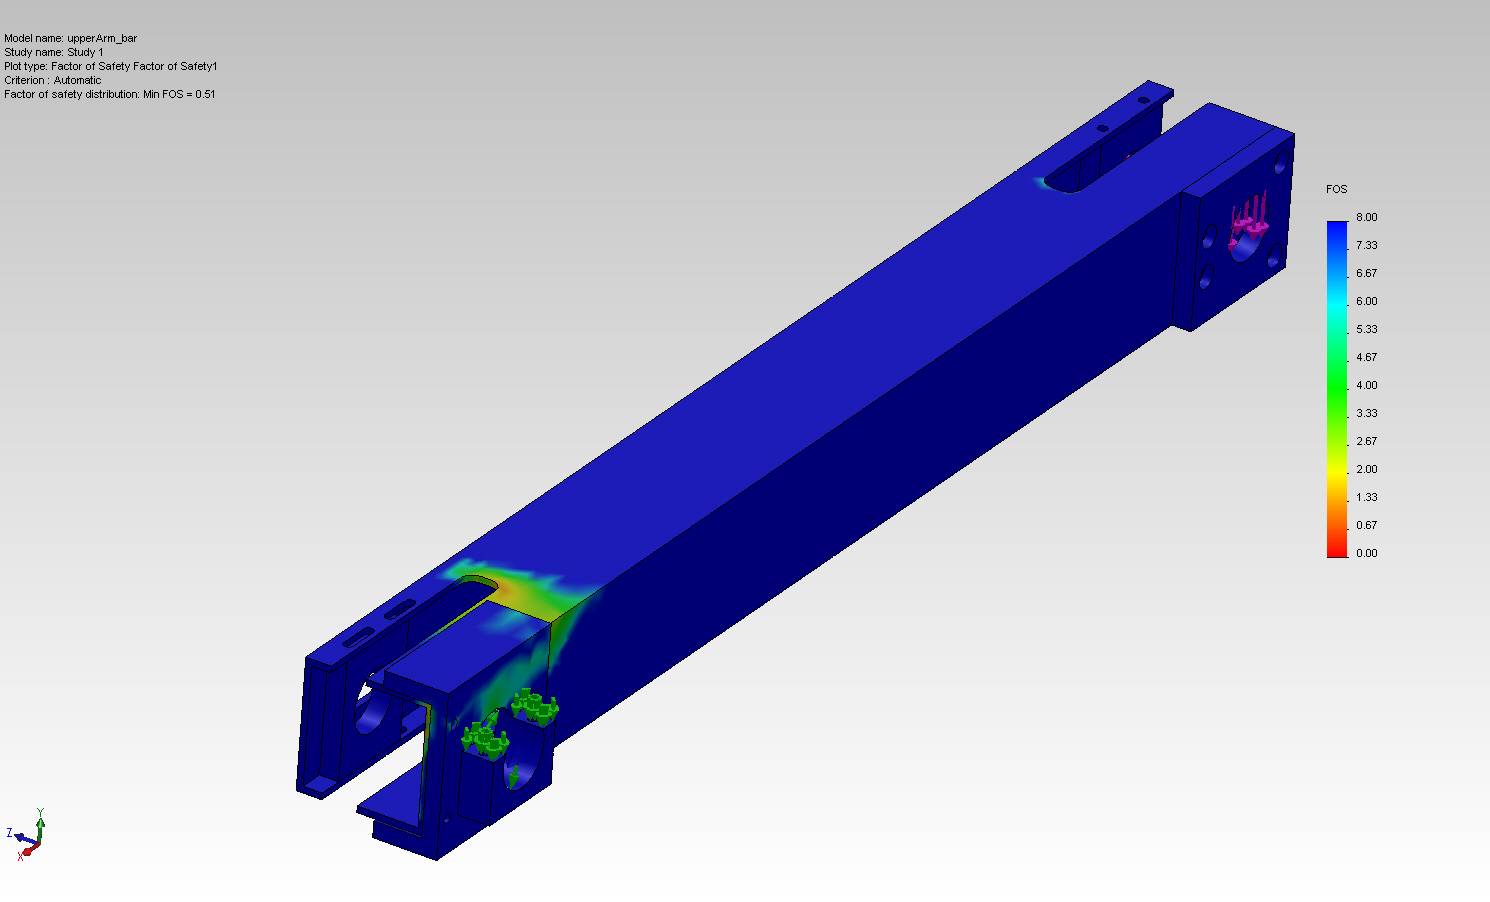
\includegraphics[scale=0.3]{Images/upperArm_bar_FOS.jpg}}
	\caption{Factor of safety plot of the upper arm}
	\label{fig:upperArm_FOS}
\end{figure}

Again it is clear that the main beam and the smaller bearing mounts are more than strong enough. However, at the edges of the slots in the main beam the safety factor decreases to almost 1. This is the reason steel was selected.

The deformation plot shows deformation up to 0.6mm, which is acceptable for our robot. If the arm could be designed without the slots it would be a lot less, and the arm could probably be made from aluminium. Because of time constrains it was decided to leave it this way, but it could be an improvement in a future version.

\begin{figure}[ht!]
	\centering
	\mbox{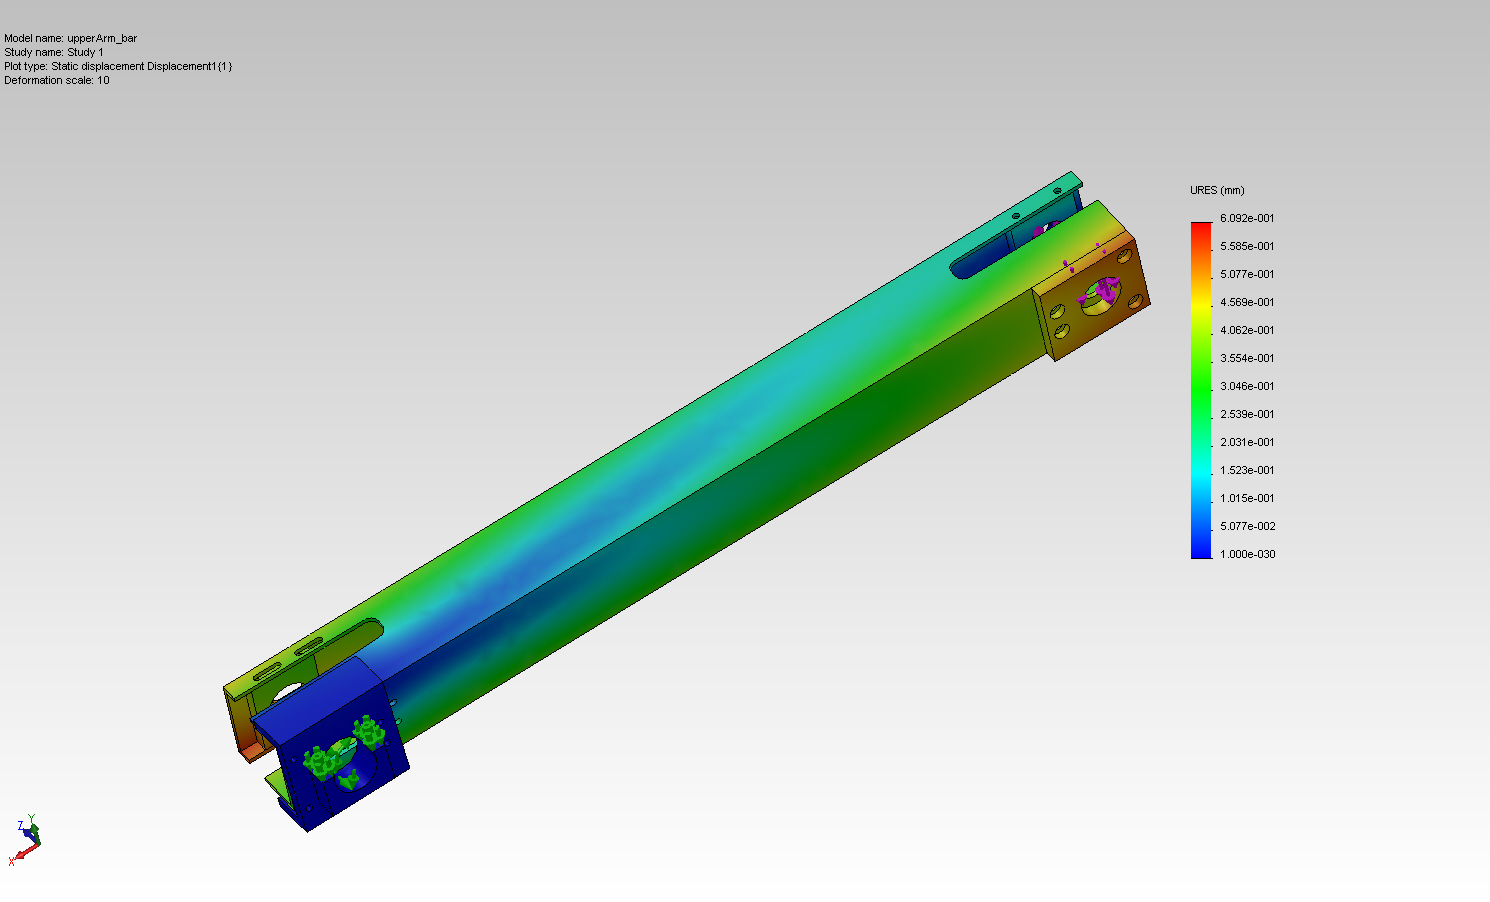
\includegraphics[scale=0.3]{Images/upperArm_bar_displace.jpg}}
	\caption{Displacement plot of the upper arm}
	\label{fig:upperArm_displace}
\end{figure}

These were the most important points. The further down the arm, the smaller the forces and the simpler the construction is. Most of those parts have been verified by simplified hand calculations. If one wishes to create a new version of Eva\textquotesingle{}s arm, doing more extensive calculations would be advisable. The arm certainly is strong enough, but it is probably possible to optimize its weight by removing redundant material.

\section{Drive train}

\begin{figure}[ht!]
	\centering
	\mbox{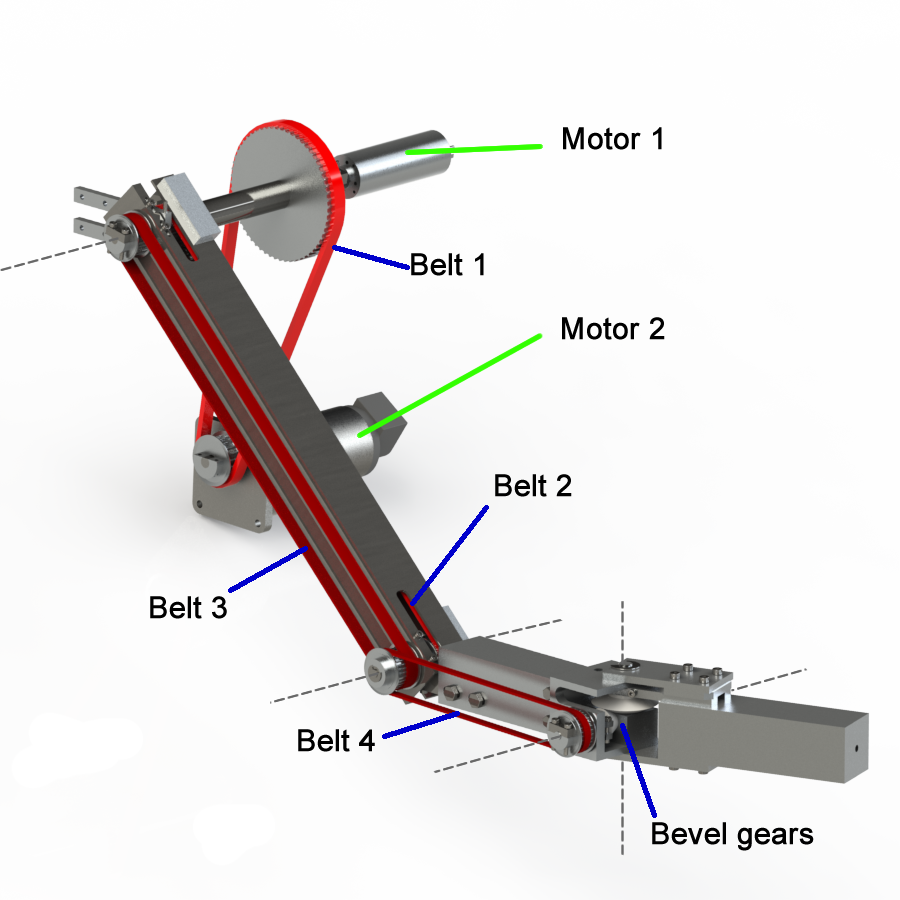
\includegraphics[scale=1.0]{Images/overview_legenda.png}}
	\caption{Overview of Eva\textquotesingle{}s arm}
	\label{fig:overviewLegenda}
\end{figure}

So far the mechanical working of the arm has been discussed. After the strength calculations the arm is confirmed to meet its requirements. However, when moving the arm or holding it up with a heavy load in its gripper, a substantial force will act on the timing belts and other drive train components. This section will discuss the selection of each of these components. See fig. \ref{fig:overviewLegenda} for an overview of the drive train.



\subsection{driving the shoulder}

For driving the shoulder joint, the required torque is at its maximum when the arm is fully stretched. As shown in fig. \ref{fig:driveTrain_shoulder} the required moment is 25Nm, assuming an object weighing $2kg$. To achieve this moment a motor and transmission had to be chosen. A motor\footnote{Motor 2 in fig. \ref{fig:overviewLegenda}} with a maximum torque of $5.6Nm$ was already available, as well as an AT5-GenIII 10*680 timing belt\footnote{Belt 1 in fig. \ref{fig:overviewLegenda}}. Some calculations were made to select a set of pulleys with the required transmission ratio, which ideally would be $1:4.5$ ($5.6Nm / 25Nm \approx 4.5$). The biggest pulley available had 60 teeth, so a pulley with 13 teeth would be optimal. However, with too few teeth in mesh with the timing belt, the tension on the timing belt\textquotesingle{}s tooth would be too large.

\begin{figure}[ht!]
	\centering
	\mbox{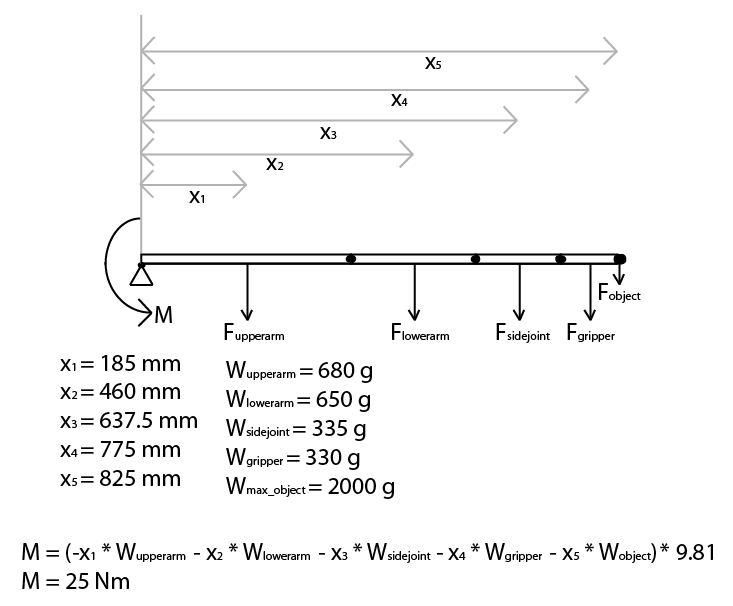
\includegraphics[scale=0.5]{Images/driveTrain_shoulder.png}}
	\caption{Calculating the moment on Eva\textquotesingle{}s shoulder}
	\label{fig:driveTrain_shoulder}
\end{figure}
 
For each of the timing belts, the required belt width was calculated using formula \ref{eq:b_tooth}. The total tension on each belt was also checked to confirm the selected belt would be sufficiently strong.

\begin{equation}
\label{eq:b_tooth}
b_{tooth} = T/(z_{1}*z_{e}*M_{spec})
\end{equation}
Where $b_{tooth}$ is the required belt width ($m$), $T$ is the pulley torque ($Nm$), $z_{1}$ the amount of teeth on the smallest pulley, $z_{e}$ the number of teeth in mesh and $M_{spec}$ the specific torque ($Nm$), supplied by the belt manufacturer. Since a $10mm$ wide belt had to be used\footnote{The shaft of the available motor was not long enough to properly fit a wider pulley}, the smallest pulley suitable for this belt size was a pulley with 20 teeth, resulting in a transmission ratio of $20:60$. The tension on the belt would be $T / r_{pulley} = 5.6Nm / 15.3*10^{-3}m = 366N$. Since this belt is capable of handling a tension force of $787N$, the belt is strong enough.

However, since the transmission ratio now is $1:3$ instead of $1:4.5$, the motor can only provide $16.8Nm$ to the shoulder joint. This means that the object which is picked up can have a maximum weight of 992 grams. This is half of the weight of the design constrain as defined on the begin of this project\footnote{The goal for the arm was to be capable of lifting objects up to $2kg$}. For this prototype 992 grams is enough, because it is more than the weight of the drinks Eva serves.

\subsection{Keeping it horizontal}

The transmission which is used to keep the lower arm horizontal consists of two pulleys and a timing belt\footnote{Belt 2 in fig. \ref{fig:overviewLegenda}}. The momentum on this timing belt is mainly caused by the weight of the object. Fig. \ref{fig:driveTrain_elbow} shows the calculation of this momentum.

\begin{figure}[ht!]
	\centering
	\mbox{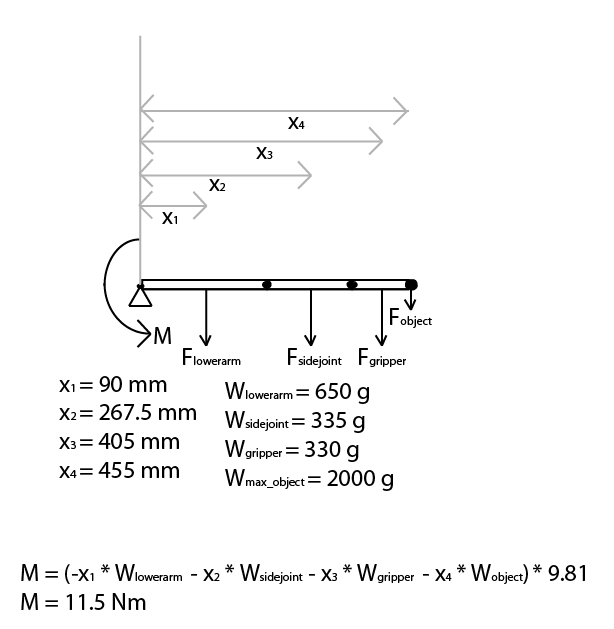
\includegraphics[scale=0.7]{Images/driveTrain_elbow.png}}
	\caption{Calculating the moment on Eva\textquotesingle{}s elbow}
	\label{fig:driveTrain_elbow}
\end{figure}

The momentum in the transmission is $11.5Nm$. To select a suitable set of pulleys and timing belt, formula \ref{eq:b_tooth} was again used. To keep the arm compact, the pulleys should be as small as possible, while capable of transferring the torque mentioned. The smallest pulleys available meeting the requirements were AT-3 pulleys with 32 teeth. In combination with an AT3-GenIII 10*816 belt they would be the perfect transmission. 

By accident a regular AT-3 belt was ordered instead of the slightly stronger AT3-GenIII timing belt. This means the allowed torque is slightly below $11.5Nm$, resulting in a maximum allowable object weight  of 1560 grams. It is below $2kg$, but as mentioned before, the shoulder transmission is the bottle neck, only being capable of lifting 992 grams.
Therefore the selected belt was considered good enough. To improve Eva\textquotesingle{}s arm, incorporating a GenIII timing belt would be reccomended.

\subsection{Moving the arm sideways}

In the design the decision was made to put the motor\footnote{Motor 1 in fig. \ref{fig:overviewLegenda}}, which is needed to move the arm sideways, in the body. So a transmission is needed from the body to the sideJoint. This transmission consists of two transmissions by timing belts\footnote{Belt 3 and 4 in fig. \ref{fig:overviewLegenda}} and one transmission by a set of bevel gears\footnote{see fig. \ref{fig:overviewLegenda}}. To calculate the torque which the motor has to deliver, a calculation of the sideways movement of the arm, gripper and object was made. The biggest torque which the motor has to deliver is estimated to be caused by the drivetrain and friction between the parts of the lowerarm and the sideJoint. This is very difficult to determine, so at first only a calculation of the moment which is cause by the inertia was made. The lower arm, gripper and object were simplified to a rectangle and a circle, as in the calculations in fig. \ref{fig:driveTrain_sideJoint}.

\begin{figure}[ht!]
	\centering
	\mbox{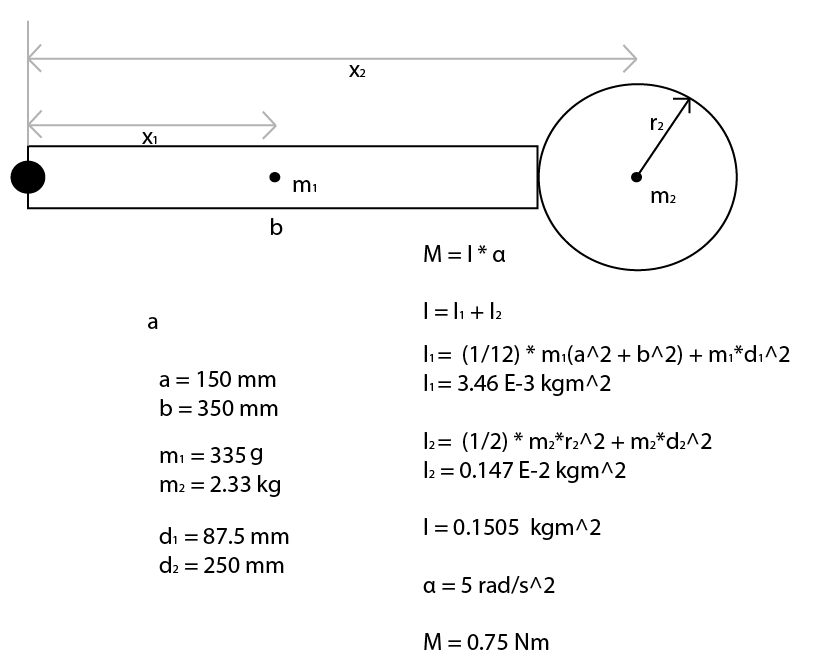
\includegraphics[scale=0.5]{Images/driveTrain_sideJoint.png}}
	\caption{Calculating the moment required to move the arm sideways}
	\label{fig:driveTrain_sideJoint}
\end{figure}

A maximum angular velocity of $5 rad/s^2$ was assumed. This resulted in a momentum of $0.75Nm$. This moment should be delivered by the bevel gears. Therefore a set of bevel gears with an allowed torque of at least $0.75Nm$ had to be selected. The chosen bevel gear is capable of providing torque up to $0.84Nm$. As the transmission ratio of this set of gears is 1:2, the torque on the smaller gear is $0.38Nm$. This is the torque that needs to be transferred from the motor, via timing belts 3 and 4 in fig. \ref{fig:overviewLegenda}. These timing belts would need to be strong enough to transfer a torque between $0.38Nm$ and $0.8Nm$, depending on how much friction would act on the drivetrain. The pulleys had to be the same diameter as those connected to belt 2 in fig. \ref{fig:overviewLegenda}, as a slightly different size would result in a different belt length that would not be available. Because of these relatively big pulleys, the tension on the belts is very low. Therefore even the smallest width of 6mm turned out to be sufficient. An overview of all drivetrain components and their load is visible in table \ref{table:belts}.


\begin{table}[h]
\begin{tabular}{| p{1.7cm} | p{1.8cm} | p{1.7cm} | p{1.8cm} | p{1.7cm} | p{1.7cm} | p{1.7cm} |}
\hline
part (see fig. \ref{fig:overviewLegenda})	&	transmission ratio	&	req. belt width (mm)	&	tension (N)	&	belt width (mm)	&	allowable tension (N)	&	allowable torque (Nm)	\\
\hline
belt 1		&	20:60	&	8.86	&	366	&	10	&	787	&			\\
belt 2		&	32:32	&	12.4	&	763	&	16	&	646	&			\\
belt 3		&	32:32	&	0.5		&	27	&	10	&	380	&			\\
belt 4		&	32:32	&	0.5		&	27	&	6	&	190	&			\\
bevel gears	&	15:30	&			&		&		&		&	0.86	\\
\hline
\end{tabular}
\caption{Overview of drivetrain components}
\label{table:belts}
\end{table}


Trough the lost torque which would be caused by transmission friction of the timing belts, gears and by other friction, the required motor torque was estimated to be $0.8Nm$. So a motor which has a minimum torque of 0.8 Nm had to be chosen. A suitable B\"{u}hler motor had to be selected, because they were affordable and the delivery time would be pretty fast. 
A list of candidates for this motor was made, as shown in table \ref{table:motors}.


\begin{table}[h]
\begin{tabular}{| p{3cm} | p{3cm} | p{3cm} | p{3cm} |}
\hline
motor series	&	rated current (A)	&	stall torque (Nmm)	&	top speed (rpm)	\\
\hline
1.61.077		&						&						&					\\
412				&	1.40				&	770					&	190				\\
413				&	1.40				&	1400				&	105				\\
414				&	0.85				&	1400				&	60				\\
415				&	0.85				&	2520				&	33				\\
\hline
1.61.050		&						&						&					\\
443				&	3.60				&	4060				&	72				\\
447				&	1.90				&	5600				&	16				\\
\hline
1.61.117		&						&						&					\\
313				&	0.49				&	600					&	55.5			\\
314				&	0.38				&	600					&	37.5			\\
315				&	0.36				&	800					&	22.5			\\

\hline
\end{tabular}
\caption{Overview of motor candidates}
\label{table:motors}
\end{table}


A tradeoff between energy consumption, available torque and speed resulted in selecting the B\"{u}hler 1.61.077.414 gearbox motor. It has a holding torque above 0.8Nm, is fast enough and does not consume too much current. To allow accurate closed-loop control of the sideways motion, a fitting encoder was ordered as well.


\subsection{Angle limits}

As the motors driving the arm have relative encoders, they need a reference point to know at which angle the arm is positioned. This is implemented by a switch on each degree of freedom. When Eva starts the main program for the first time, she moves her arm slowly to those switches. When the switches detect they are hit, the current position is saved. This ensures the arm always knows where it is. To prevent the arm from colliding with itself, these angle limits are implemented in Eva\textquotesingle{}s software.

A second set of switches is placed close to the physical limits. If for some reason the arm moves beyond its software limits, these switches send an emergency signal to the threemixel to ensure the motors immediately stop turning. This system prevents damage to the arm; its only purpose is safety. Note that the arm will not move as long as it is at its angle limits and has to be moved manually before the threemixel will allow further movement. Under normal operation this situation does not occur, but especially while testing new software it has proven to be a very useful feature.


\end{document}